\section{System Design}

\subsection{System Overview}
Determining the overall design of the system was initially hard since it was not clear exactly how many subsystems would be needed to mesh, evaluate and interface with LISA, what was clear was that the system would essentially be performing an optimisation procedure and as such needed to be driven iteratively towards a goal. The complexity and uncertainty surrounding the project meant ensuring the architecture remained modular was essential with well defined interfaces allowing components could easily be added or modified as the project progressed. \\ 

\begin{figure}[!h]
  \centerline{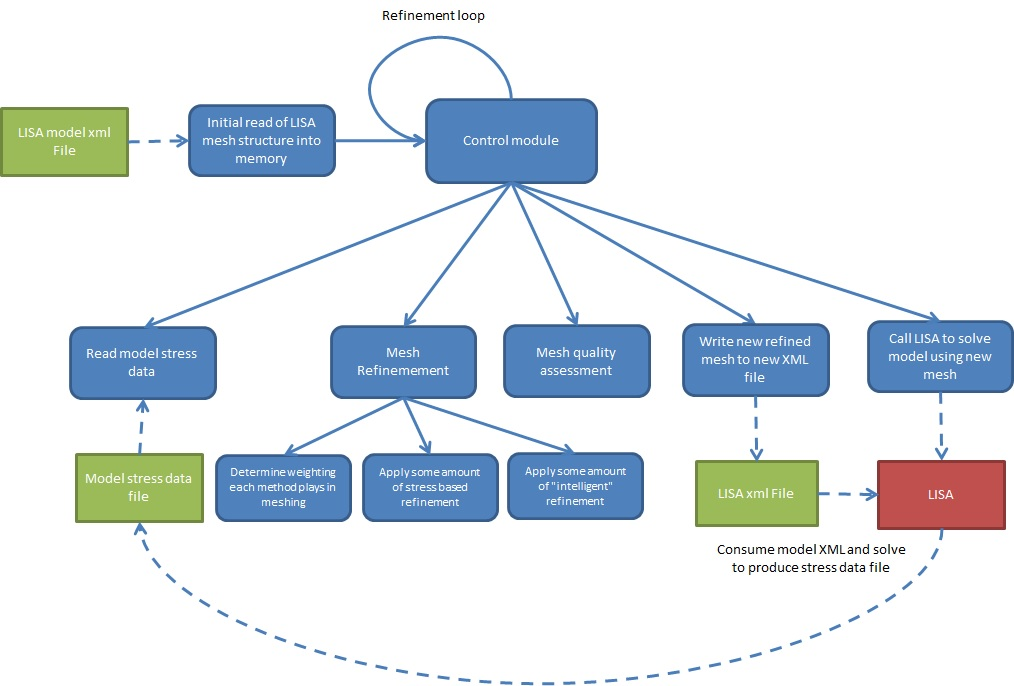
\includegraphics[width=150mm, scale=1]{../Graphics/SystemDesignDiagram.jpeg}}
  \caption{High level design of the system with its different modules}
  \label{fig:h-refinementImp}
\end{figure}


\subsection{Modular Architecture}
The modular architecture allows meshing algorithms and metrics for calculating mesh quality could be swapped interchanged was an important consideration in the design of the system. At best the quality of the output could be predicted for each method before it was integrated into the system and executed in a range of different scenarios. To have tightly coupled these individual components would have rendered the overall system a failure in the event that any one of them performed greatly worse than expected. Instead the loose coupling of the architecture has enabled the system to be considered as more of a framework for testing the effects of combining heuristic knowledge of a Finite element problem with a stress based refinement method.\\

\noindent
Although the system was highly modular It was also still desirable to maintain a hierarchy within the classes so that smaller components could be developed independently and contained within the larger ones. Composition was therefore generally favoured over inheritance as a means of building the architecture. Static classes and methods were also used when needing to write utility functions that were required by multiple high level subsystems and therefore did no fit especially well into any particular one. Examples of these are generic vector algebra operations such as dot product, matrix determinants and normal vectors.

%\subsection{Mesh improvement Loop}
%As with many optimisation problems the refinement process is driven iteratively through a loop. Within the main loop all %interfacing with LISA, Mesh refinement and analysis is conducted which results in an updated version of the model that can be %handed to the subsequent iteration.


\subsection{Input Files}
The system requires three basic input files which should be placed within a directory that is given to the program as as parameter, these are files are:

\begin{itemize}
\item A structural model represented as a .liml file which LISA can solve
\item An initial stress data file generated manually so the system has some idea about where to start working
\item A JSON file containing important edges as identified by an engineer 
along with associated meta data.
\end{itemize}

An example of the content and format for each of these input files can be seen in Appendix B

\subsection{Simulation Data Model}
Writing an API for LISA was the first clear stage of development for my project for which a design had to be considered. The API was crucial in order to program the more complex aspects using basic operations and avoid having to regularly perform direct string manipulation of the input files in order to manipulate the model. \\

\noindent
When the first re-meshing iteration occurs the system needs to read the input .liml file into an equivalent class model which closely resembles the schema specified within the .liml file, diagrams for which can be seen in figure 4 below. Each class in this model contains corresponding data and methods used to represent and manipulate the model. These methods are then used by the different refinement methods that exist in the different optimisation classes to alter the mesh, this adapted version of the mesh represented as a data model can then be assessed by the module responsible for validating mesh quality before finally being written back to a .liml file for LISA to solve on the subsequent iteration. When designing the data model to represent the state within LISA it was desirable to maintain coherence with the structure specified by LISA as closely as possible, this allowed for the data model to more easily be serialised when communicating with LISA without errors resulting from inconsistencies between the two representations. 

\begin{figure}[!h]
\centering
\begin{subfigure}{.5\textwidth}
  \centering
  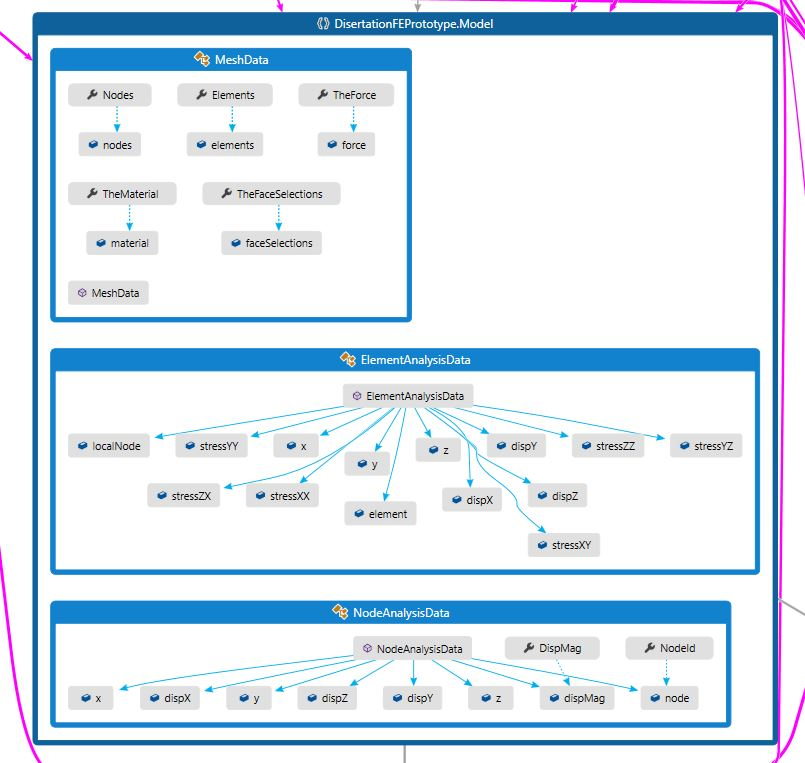
\includegraphics[width=0.9\linewidth]{../Graphics/DissoFEProto-Model.jpg}
  \caption{Model classes}
  \label{fig:sub1}
\end{subfigure}%
\begin{subfigure}{.5\textwidth}
  \centering
  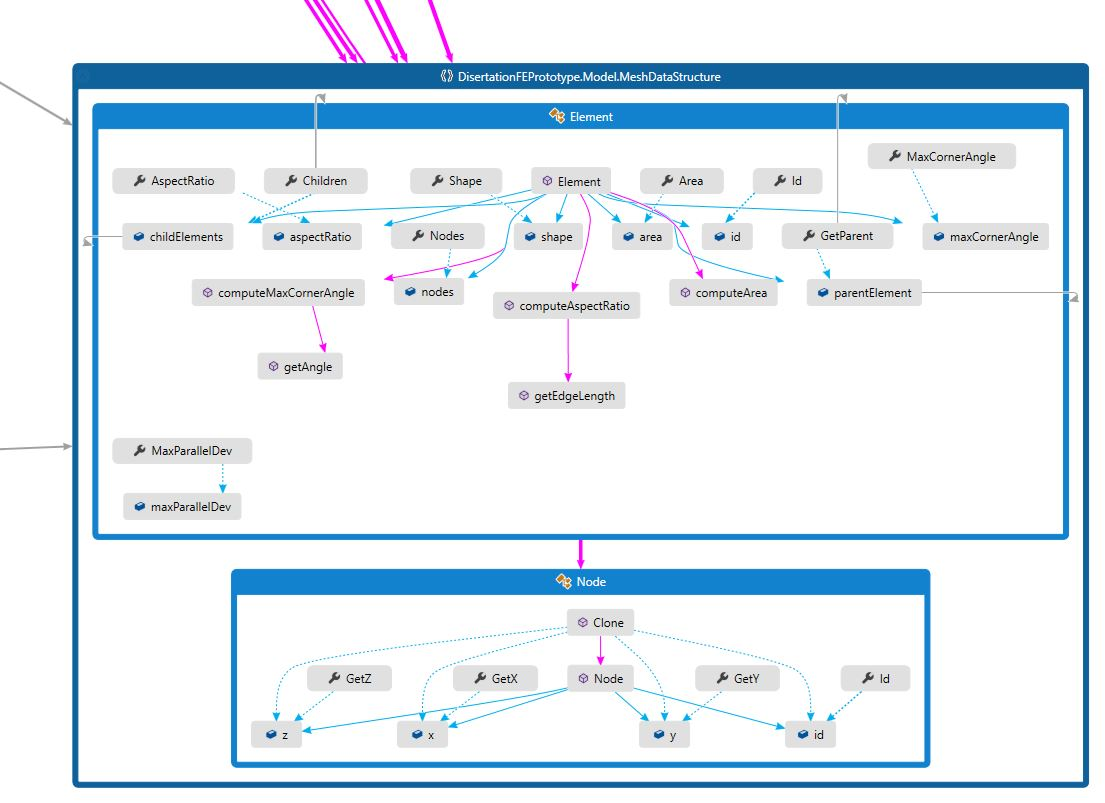
\includegraphics[width=0.9\linewidth]{../Graphics/DissoFEProto-ElemNode.jpg}
  \caption{Element and Node classes}
  \label{fig:sub2}
\end{subfigure}
\label{fig:test}
\end{figure}

\begin{figure}
\centering
\begin{subfigure}{.5\textwidth}
  \centering
  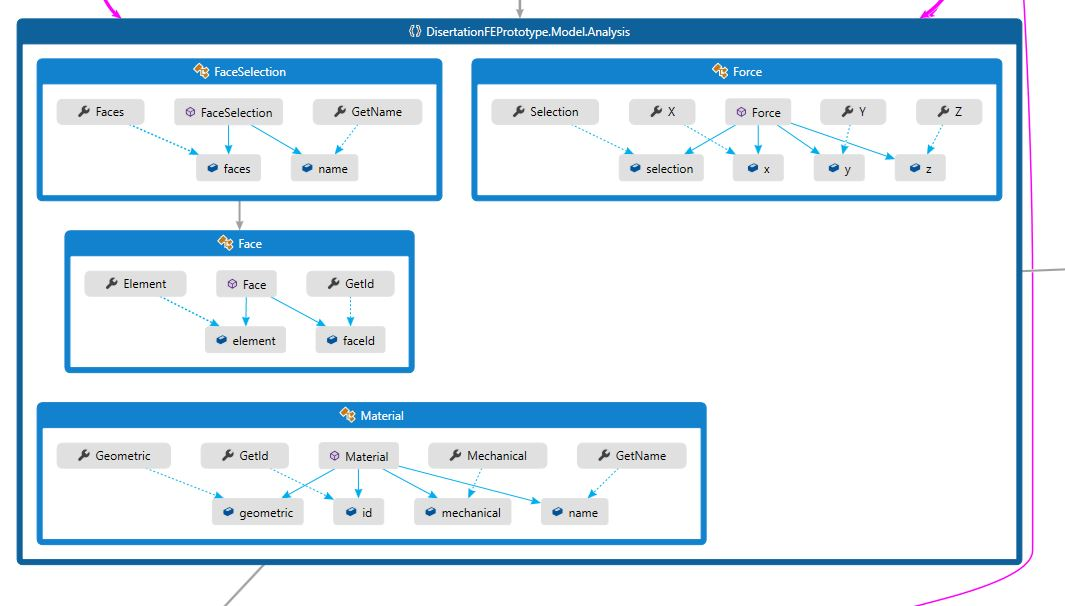
\includegraphics[width=0.9\linewidth]{../Graphics/DissoFEProto-ModelAnalysis.jpg}
  \caption{Model Analysis classes}
  \label{fig:sub1}
\end{subfigure}%
\begin{subfigure}{.5\textwidth}
  \centering
  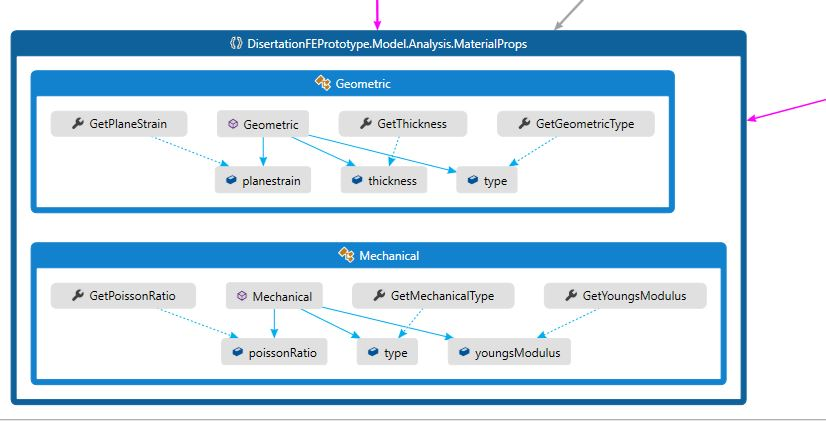
\includegraphics[width=0.9\linewidth]{../Graphics/DissoFEProto-MaterialProps.jpg}
  \caption{Material Property classes}
  \label{fig:sub2}
\end{subfigure}
\label{fig:test}
\caption{Class model to represent .liml file structure used by LISA}
\end{figure}

\noindent
One aspect of the data models design which greatly adds to the systems flexibility is the hierarchical design for representing the various Element types. At the root of this structure is the IElement interface, all new Element types must adhere to this in order for the various refinement methods to run. Implementing the interface are a range of abstract classes such as ``SquareBasedElem" and ``TriangleBasedElem" These classes are designed to contain methods that are generally applicable for calculating metrics and re meshing individual elements for elements of this type that are both in two and three dimensions. This is powerful since computing this for a 3d element is simply a reduction of the method for a 2d element over every face which comprises the 3d one. Finally underneath this level are the concrete classes which represent each specific type of element with its own bespoke characteristics. \\ 

\begin{figure}[!h]                                                   
  \centerline{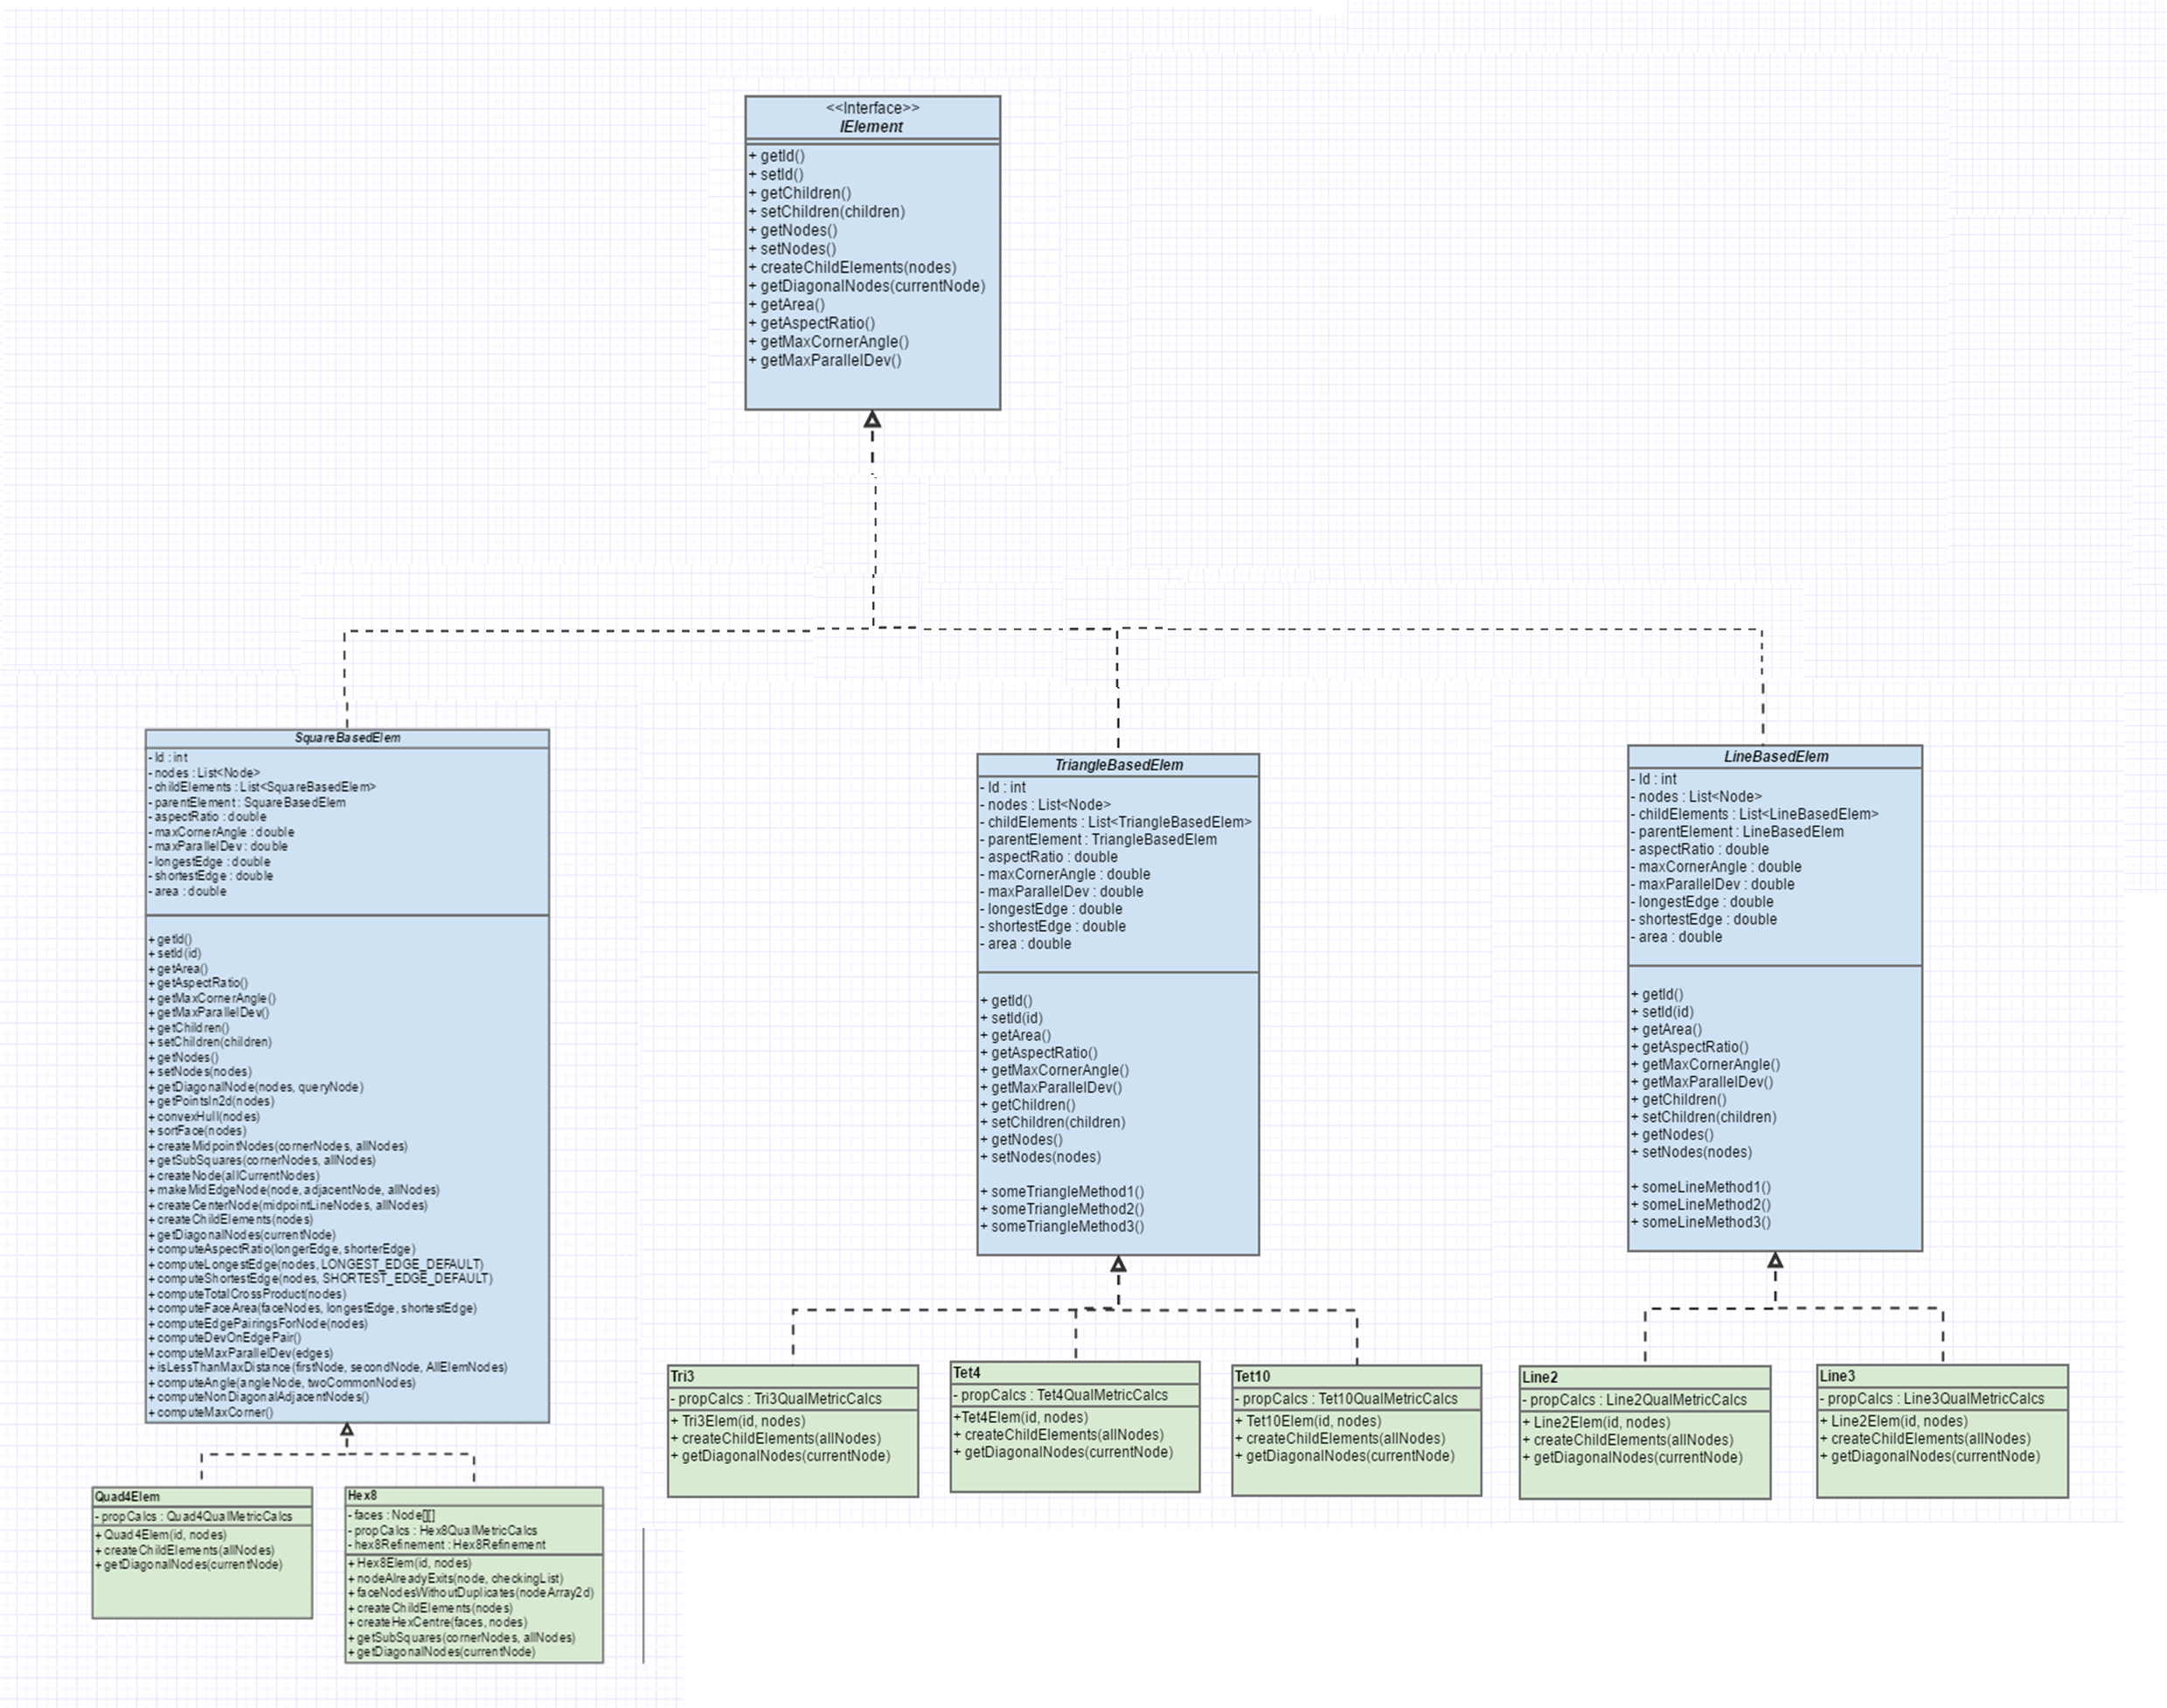
\includegraphics[width=150mm, scale=1]{../Graphics/ElementHigerarchyDiagram2.png}}
  \caption{Class diagram showing the hierarchy of element classification within the data model, due to time limitations I was not able to implement the respective classes for triangle and line based elements, to see image representations of each element type within this class diagram refer to element type appendix}
  \label{fig:h-refinementImp}
\end{figure}


\subsection{Remeshing methods approach}
Due to the modular design of the system the low level methods for performing refinement for each element type were contained within the elements abstract class or if more bespoke its subclass, see Figure 6. This made it much easier to decouple both the stress and heuristic methods allowing each of them to simply have the task of selecting elements which they considered beneficial to refine before delegating the refinement to each element itself. This allowed both high level refinement approaches to utilise the same low level functionality which greatly improved the systems reliability and simplified the design.

\subsubsection{Combining methods}
Since each refinement method could be executed independently of the other it made sense when testing combinations both to simply enumerate the combinations that each could be applied for each iteration before running each specific combination iteratively on a model. This results in a set of two valued tuples up to some value :

\[ \left\{ (a, b) \,\middle|\, \, a,b \in \mathbb{N} a,b < k \right\} \]


\subsubsection{Multi Threading}
To allow allow for better performance when evaluating a range of different weightings of the stress and heuristic methods multi threading was used to allow each configuration to be run independently of the others. When started each thread creates its own directory which it copies the three input files to and runs for its designating weighting configuration. \colorbox{yellow}
{Use of multi threading made assessment of the system much more rapid in the later stages of the project with the overall execution time being reduced from x to x equalling a speed up of y}
